\section{Application architecture}
\label{sec:application-architecture}

	\subsection{Prototypical application structure}
	
	This section presents the application architecture from the solution architecture point of view. A generic solution architecture is depicted in Figure \ref{fig:application-view}.
	
	The application architecture we present here takes the form of a 
	
    \begin{figure}[h]
		\centering
		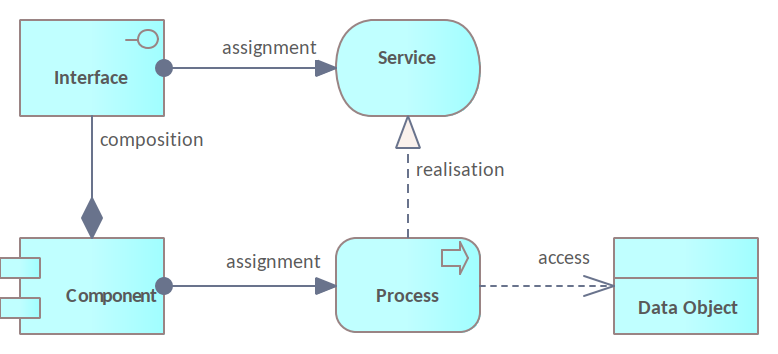
\includegraphics[width=.9\textwidth]{docs/architecture/images/views/Application view.png}
		\caption{The prototypical application structure view}
		\label{fig:application-view}
	\end{figure}
	
	\subsection{Current application service architecture}
	\label{sec:application-current}
	
	\begin{figure}[h]
		\centering
		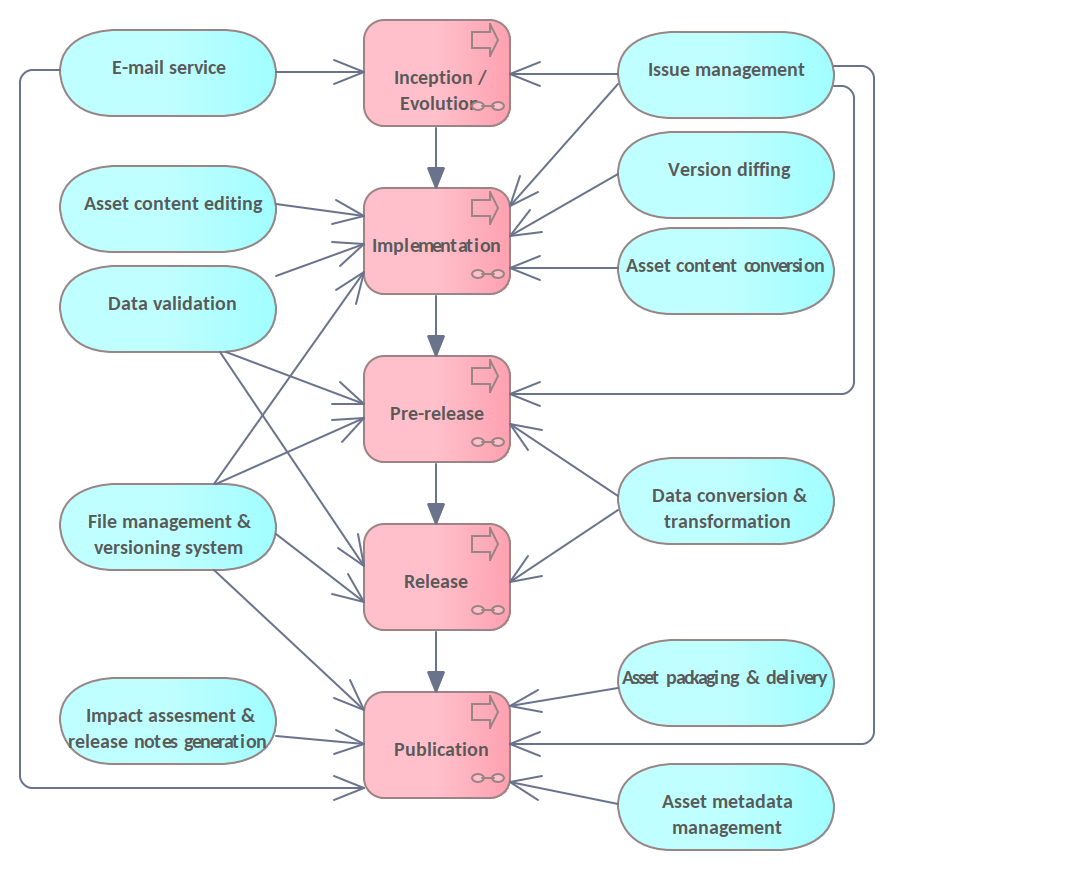
\includegraphics[width=.9\textwidth]{images/application/Application Services (current).png}
		\caption{The application services that serve the current asset lifecycle}
		\label{fig:application-current}
	\end{figure}
	
	\subsection{New application service architecture}
	\label{sec:application-new}	

	\begin{figure}[h]
		\centering
		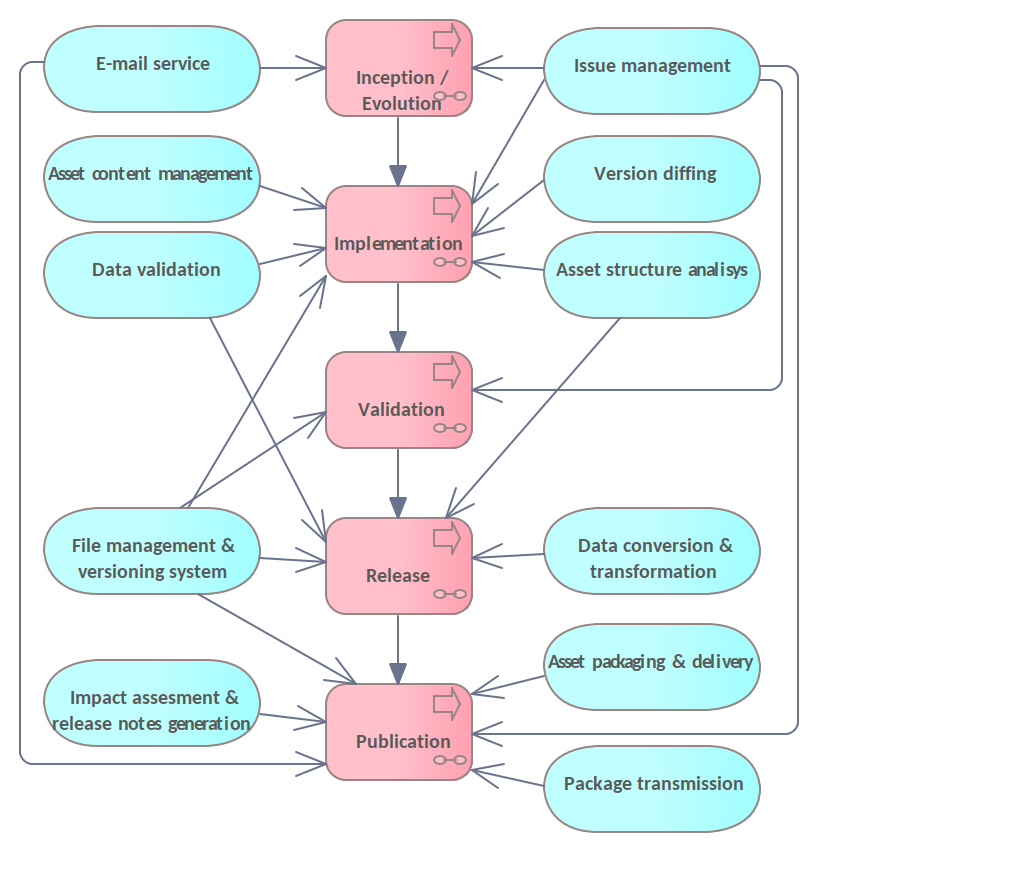
\includegraphics[width=.9\textwidth]{images/application/Application Services (new).png}
		\caption{The application services that serve the new asset lifecycle}
		\label{fig:application-new}
	\end{figure}	
	
	\subsection{Inception and evolution services and components}
	\label{sec:evolution-application}	
	\begin{figure}[h]
		\centering
		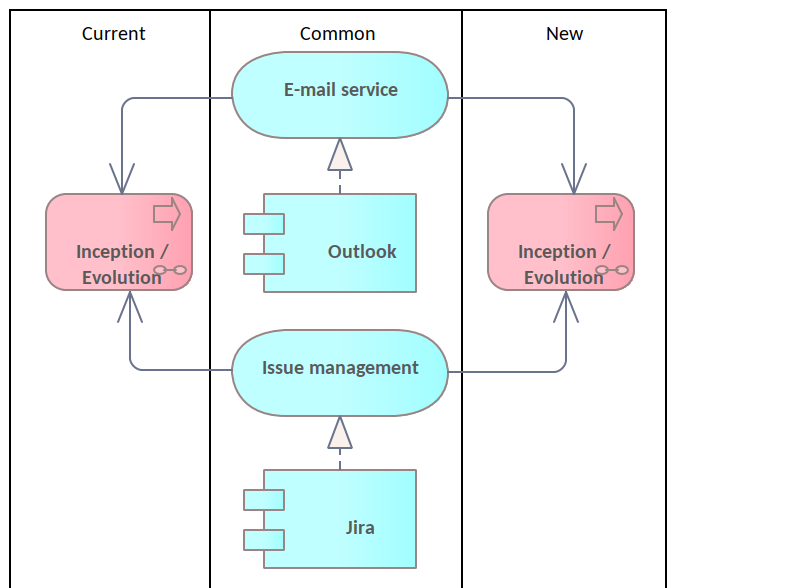
\includegraphics[width=.6\textwidth]{images/application/InceptionEvolution.png}
		\caption{The application services and components that serve the current and new inception and evolution stage}
		\label{fig:application-inception-evolution}
	\end{figure}

	\subsection{Implementation services and components}
	\label{sec:implementation-application}	
	\begin{figure}[h]
		\centering
		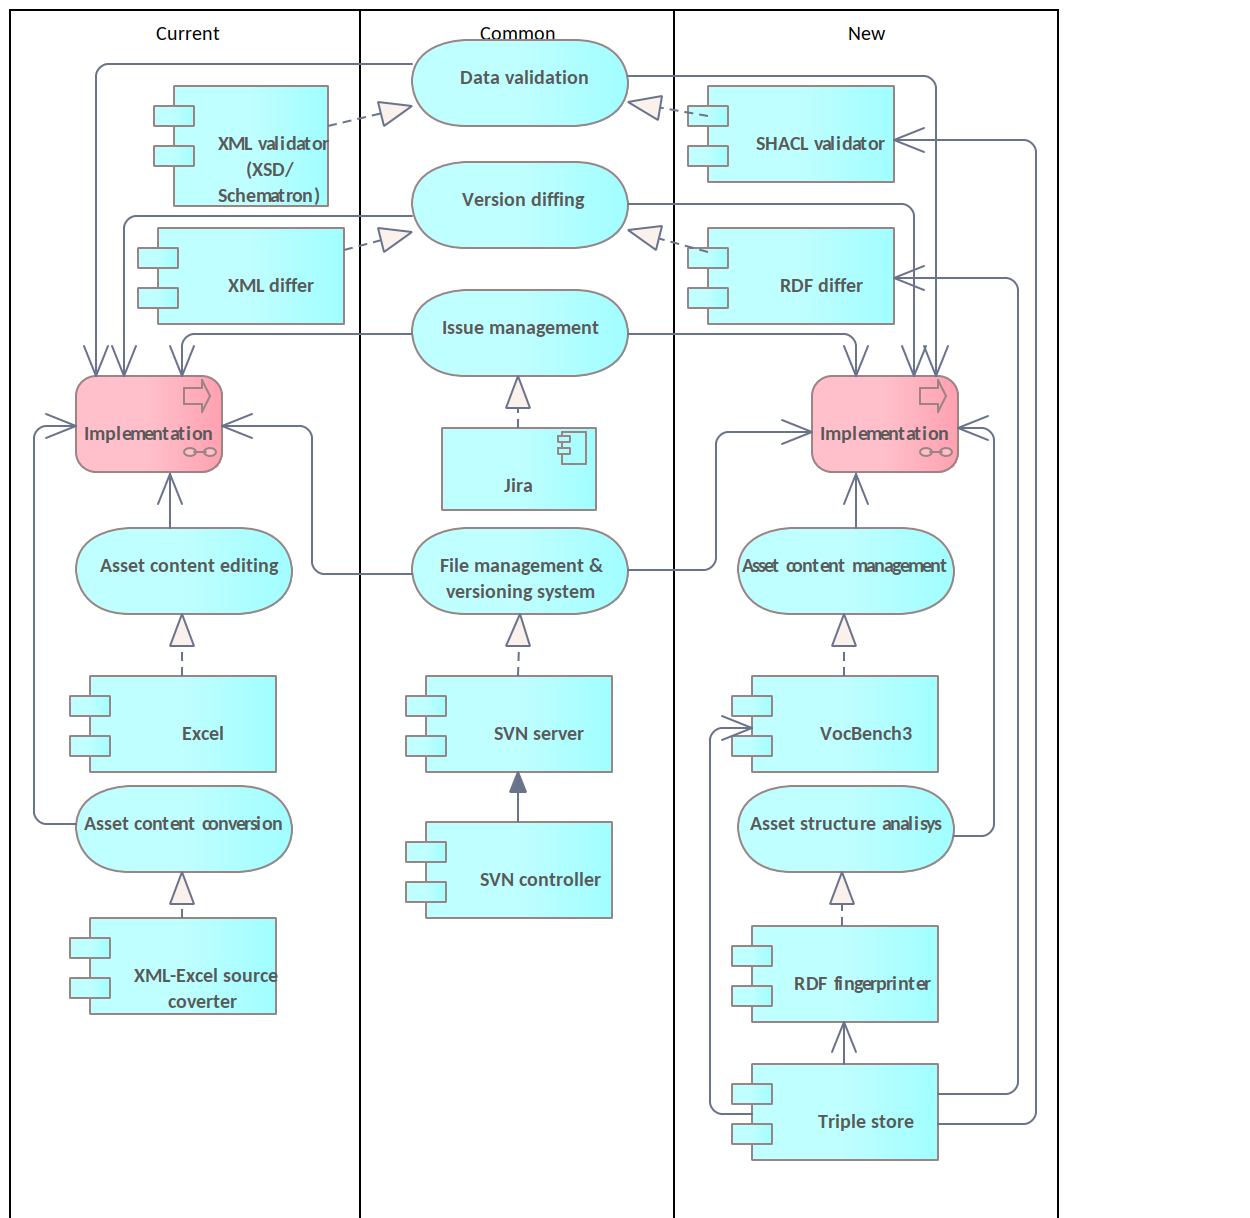
\includegraphics[width=.9\textwidth]{images/application/Implementation v3.png}
		\caption{The application services and components that serve the current and new implementation stage}
		\label{fig:application-implementation}
	\end{figure}
	
	\subsection{Pre-release and validation services and components}
	\label{sec:validation-application}
	\begin{figure}[h]
		\centering
		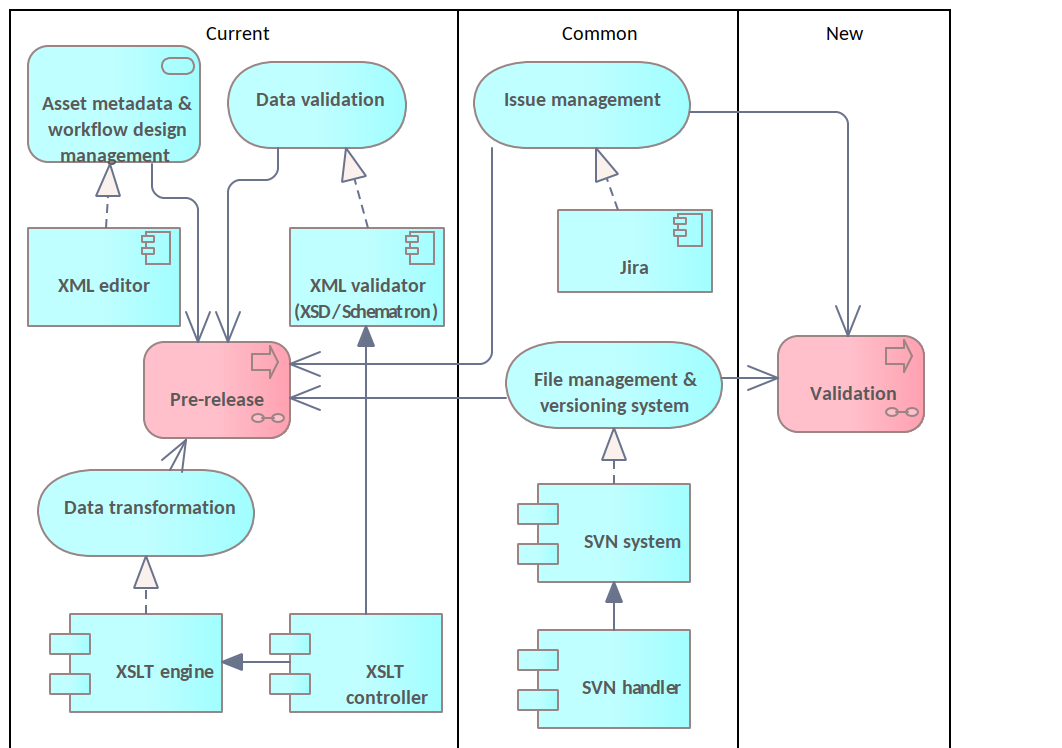
\includegraphics[width=.9\textwidth]{images/application/Validation & Pre-release v3.png}
		\caption{The application services and components that serve the current pre-release and the new validation stages}
		\label{fig:application-validation}
	\end{figure}

	\subsection{Release services and components}
	\label{sec:release-application}	
	
	\begin{figure}[h]
		\centering
		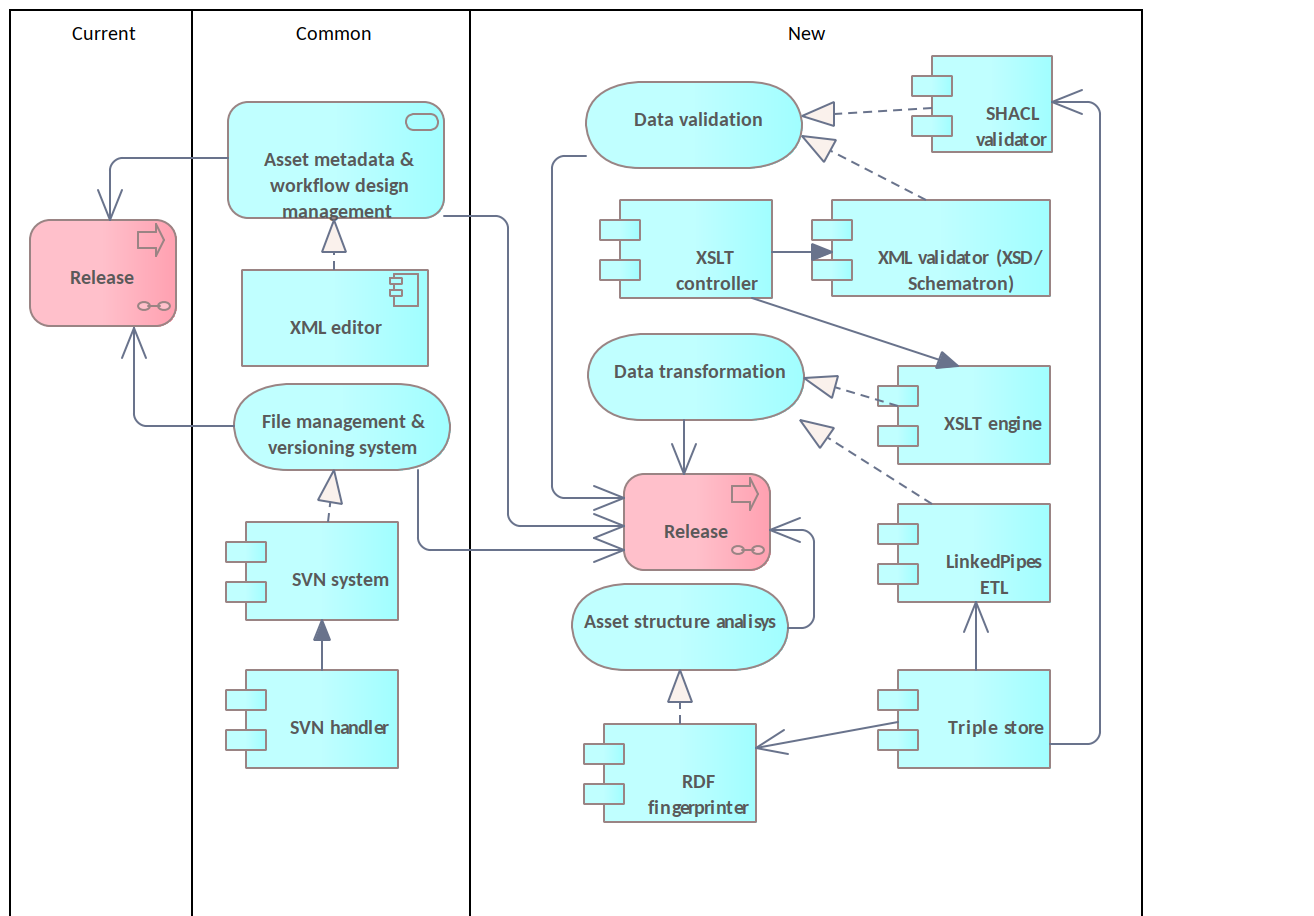
\includegraphics[width=.9\textwidth]{images/application/Release v3.png}
		\caption{The application services and components that serve the current and new release stage}
		\label{fig:application-release}
	\end{figure}
	
	\subsection{Publication services and components}
	\label{sec:publication-application}	
	
	\begin{figure}[h]
		\centering
		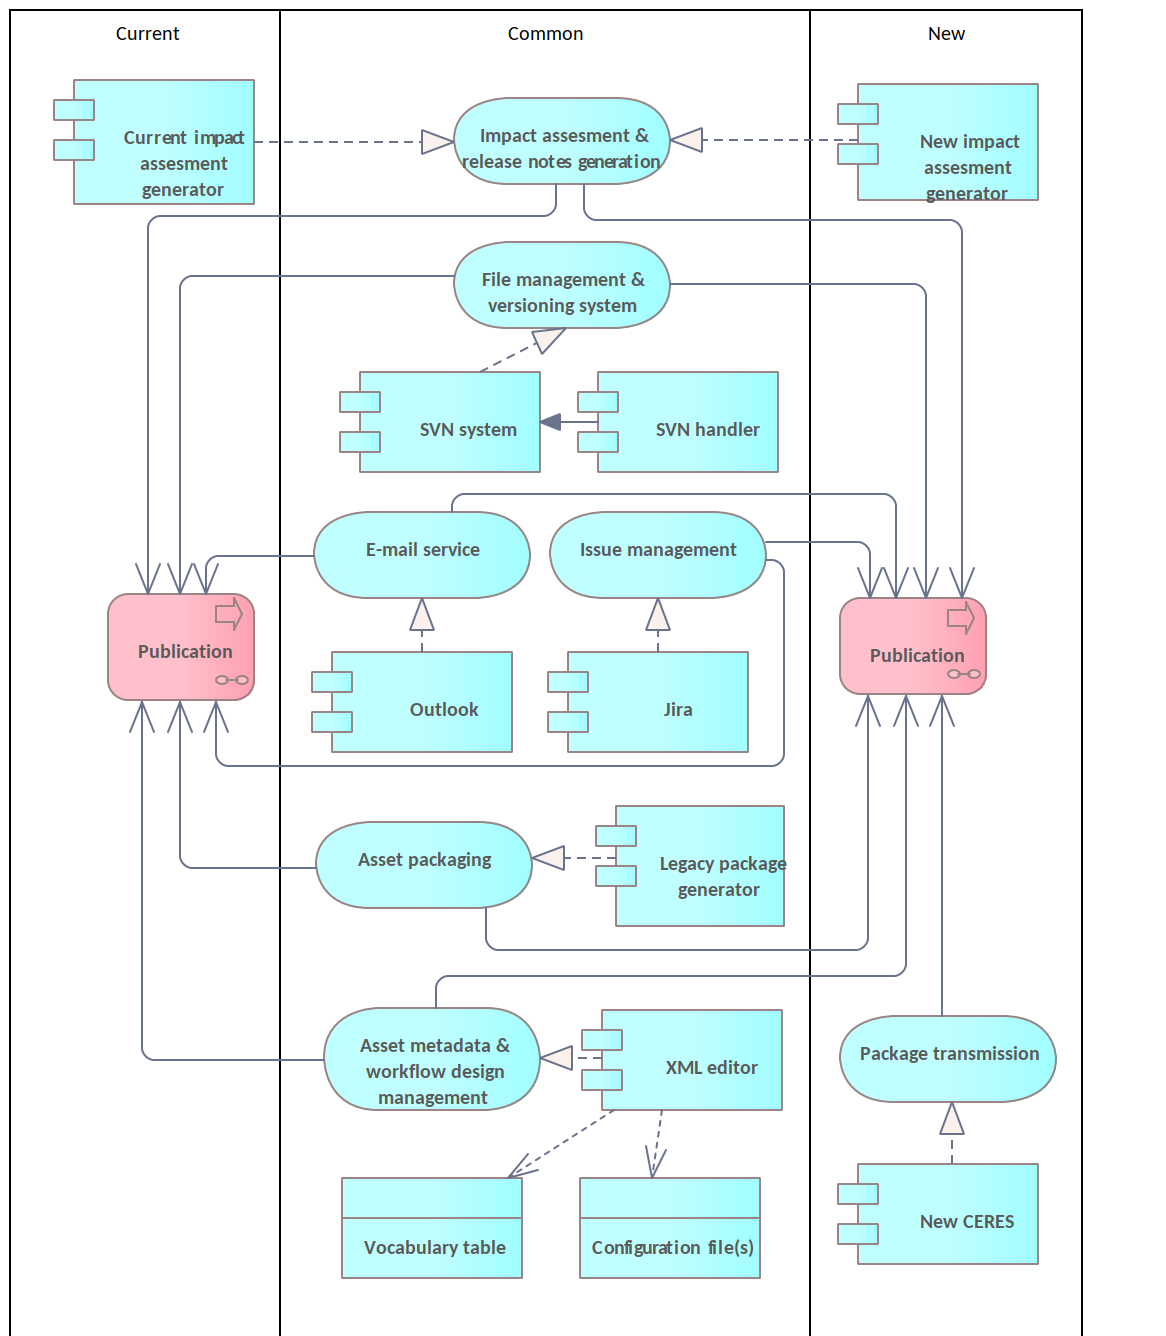
\includegraphics[width=.9\textwidth]{images/application/Publication v3.png}
		\caption{The application services and components that serve the current and new publication stage}
		\label{fig:application-publication}
	\end{figure}

	